% Options for packages loaded elsewhere
\PassOptionsToPackage{unicode}{hyperref}
\PassOptionsToPackage{hyphens}{url}
\PassOptionsToPackage{dvipsnames,svgnames,x11names}{xcolor}
%
\documentclass[
  11pt,
  a4paper,
]{article}

\usepackage{amsmath,amssymb}
\usepackage{setspace}
\usepackage{iftex}
\ifPDFTeX
  \usepackage[T1]{fontenc}
  \usepackage[utf8]{inputenc}
  \usepackage{textcomp} % provide euro and other symbols
\else % if luatex or xetex
  \usepackage{unicode-math}
  \defaultfontfeatures{Scale=MatchLowercase}
  \defaultfontfeatures[\rmfamily]{Ligatures=TeX,Scale=1}
\fi
\usepackage{lmodern}
\ifPDFTeX\else  
    % xetex/luatex font selection
    \setmainfont[]{Latin Modern Roman}
    \setsansfont[]{Latin Modern Roman}
\fi
% Use upquote if available, for straight quotes in verbatim environments
\IfFileExists{upquote.sty}{\usepackage{upquote}}{}
\IfFileExists{microtype.sty}{% use microtype if available
  \usepackage[]{microtype}
  \UseMicrotypeSet[protrusion]{basicmath} % disable protrusion for tt fonts
}{}
\usepackage{xcolor}
\usepackage[top=2.5cm,bottom=2.5cm,left=2.5cm,right=2.5cm]{geometry}
\setlength{\emergencystretch}{3em} % prevent overfull lines
\setcounter{secnumdepth}{5}
% Make \paragraph and \subparagraph free-standing
\makeatletter
\ifx\paragraph\undefined\else
  \let\oldparagraph\paragraph
  \renewcommand{\paragraph}{
    \@ifstar
      \xxxParagraphStar
      \xxxParagraphNoStar
  }
  \newcommand{\xxxParagraphStar}[1]{\oldparagraph*{#1}\mbox{}}
  \newcommand{\xxxParagraphNoStar}[1]{\oldparagraph{#1}\mbox{}}
\fi
\ifx\subparagraph\undefined\else
  \let\oldsubparagraph\subparagraph
  \renewcommand{\subparagraph}{
    \@ifstar
      \xxxSubParagraphStar
      \xxxSubParagraphNoStar
  }
  \newcommand{\xxxSubParagraphStar}[1]{\oldsubparagraph*{#1}\mbox{}}
  \newcommand{\xxxSubParagraphNoStar}[1]{\oldsubparagraph{#1}\mbox{}}
\fi
\makeatother


\providecommand{\tightlist}{%
  \setlength{\itemsep}{0pt}\setlength{\parskip}{0pt}}\usepackage{longtable,booktabs,array}
\usepackage{calc} % for calculating minipage widths
% Correct order of tables after \paragraph or \subparagraph
\usepackage{etoolbox}
\makeatletter
\patchcmd\longtable{\par}{\if@noskipsec\mbox{}\fi\par}{}{}
\makeatother
% Allow footnotes in longtable head/foot
\IfFileExists{footnotehyper.sty}{\usepackage{footnotehyper}}{\usepackage{footnote}}
\makesavenoteenv{longtable}
\usepackage{graphicx}
\makeatletter
\def\maxwidth{\ifdim\Gin@nat@width>\linewidth\linewidth\else\Gin@nat@width\fi}
\def\maxheight{\ifdim\Gin@nat@height>\textheight\textheight\else\Gin@nat@height\fi}
\makeatother
% Scale images if necessary, so that they will not overflow the page
% margins by default, and it is still possible to overwrite the defaults
% using explicit options in \includegraphics[width, height, ...]{}
\setkeys{Gin}{width=\maxwidth,height=\maxheight,keepaspectratio}
% Set default figure placement to htbp
\makeatletter
\def\fps@figure{htbp}
\makeatother
% definitions for citeproc citations
\NewDocumentCommand\citeproctext{}{}
\NewDocumentCommand\citeproc{mm}{%
  \begingroup\def\citeproctext{#2}\cite{#1}\endgroup}
\makeatletter
 % allow citations to break across lines
 \let\@cite@ofmt\@firstofone
 % avoid brackets around text for \cite:
 \def\@biblabel#1{}
 \def\@cite#1#2{{#1\if@tempswa , #2\fi}}
\makeatother
\newlength{\cslhangindent}
\setlength{\cslhangindent}{1.5em}
\newlength{\csllabelwidth}
\setlength{\csllabelwidth}{3em}
\newenvironment{CSLReferences}[2] % #1 hanging-indent, #2 entry-spacing
 {\begin{list}{}{%
  \setlength{\itemindent}{0pt}
  \setlength{\leftmargin}{0pt}
  \setlength{\parsep}{0pt}
  % turn on hanging indent if param 1 is 1
  \ifodd #1
   \setlength{\leftmargin}{\cslhangindent}
   \setlength{\itemindent}{-1\cslhangindent}
  \fi
  % set entry spacing
  \setlength{\itemsep}{#2\baselineskip}}}
 {\end{list}}
\usepackage{calc}
\newcommand{\CSLBlock}[1]{\hfill\break\parbox[t]{\linewidth}{\strut\ignorespaces#1\strut}}
\newcommand{\CSLLeftMargin}[1]{\parbox[t]{\csllabelwidth}{\strut#1\strut}}
\newcommand{\CSLRightInline}[1]{\parbox[t]{\linewidth - \csllabelwidth}{\strut#1\strut}}
\newcommand{\CSLIndent}[1]{\hspace{\cslhangindent}#1}

\usepackage{booktabs}
\usepackage{longtable}
\usepackage{array}
\usepackage{multirow}
\usepackage{wrapfig}
\usepackage{float}
\usepackage{colortbl}
\usepackage{pdflscape}
\usepackage{tabu}
\usepackage{threeparttable}
\usepackage{threeparttablex}
\usepackage[normalem]{ulem}
\usepackage{makecell}
\usepackage{xcolor}
\usepackage{fancyhdr}
\usepackage{amsmath}
\usepackage{multirow}
\usepackage{booktabs}
\usepackage{pifont}
\makeatletter
\@ifpackageloaded{caption}{}{\usepackage{caption}}
\AtBeginDocument{%
\ifdefined\contentsname
  \renewcommand*\contentsname{Table of contents}
\else
  \newcommand\contentsname{Table of contents}
\fi
\ifdefined\listfigurename
  \renewcommand*\listfigurename{List of Figures}
\else
  \newcommand\listfigurename{List of Figures}
\fi
\ifdefined\listtablename
  \renewcommand*\listtablename{List of Tables}
\else
  \newcommand\listtablename{List of Tables}
\fi
\ifdefined\figurename
  \renewcommand*\figurename{Figure}
\else
  \newcommand\figurename{Figure}
\fi
\ifdefined\tablename
  \renewcommand*\tablename{Table}
\else
  \newcommand\tablename{Table}
\fi
}
\@ifpackageloaded{float}{}{\usepackage{float}}
\floatstyle{ruled}
\@ifundefined{c@chapter}{\newfloat{codelisting}{h}{lop}}{\newfloat{codelisting}{h}{lop}[chapter]}
\floatname{codelisting}{Listing}
\newcommand*\listoflistings{\listof{codelisting}{List of Listings}}
\makeatother
\makeatletter
\makeatother
\makeatletter
\@ifpackageloaded{caption}{}{\usepackage{caption}}
\@ifpackageloaded{subcaption}{}{\usepackage{subcaption}}
\makeatother

\ifLuaTeX
  \usepackage{selnolig}  % disable illegal ligatures
\fi
\usepackage{bookmark}

\IfFileExists{xurl.sty}{\usepackage{xurl}}{} % add URL line breaks if available
\urlstyle{same} % disable monospaced font for URLs
\hypersetup{
  pdftitle={Estimation of Effects of Endogenous Time-Varying Covariates: A Comparison Of Multilevel Linear Modeling and Generalized Estimating Equations},
  pdfauthor={Ward B. Eiling (9294163)},
  colorlinks=true,
  linkcolor={blue},
  filecolor={Maroon},
  citecolor={Blue},
  urlcolor={Blue},
  pdfcreator={LaTeX via pandoc}}


\title{Estimation of Effects of Endogenous Time-Varying Covariates: A
Comparison Of Multilevel Linear Modeling and Generalized Estimating
Equations}
\usepackage{etoolbox}
\makeatletter
\providecommand{\subtitle}[1]{% add subtitle to \maketitle
  \apptocmd{\@title}{\par {\large #1 \par}}{}{}
}
\makeatother
\subtitle{Research Report}
\author{Ward B. Eiling (9294163)}
\date{December 13, 2024}

\begin{document}
\cleardoublepage
\thispagestyle{empty}
{\centering
\hbox{}\vskip 0cm plus 1fill
% \vspace{25ex}
{\Large\bfseries Estimation of Effects of Endogenous Time-Varying
Covariates: A Comparison Of Multilevel Linear Modeling and Generalized
Estimating Equations \par}
\vspace{3ex}
{\large Research Report \par}
\vspace{9ex}
{\large\bfseries Ward B. Eiling (9294163) \par}
\vspace{3ex}
% {\Large ORCID: 0009-0007-8114-9497 \par}
% \vspace{3ex}
{\large Supervisors: Ellen Hamaker and Jeroen Mulder \par}
% \vskip 0cm plus 2fill
\vspace{9ex}
{\normalsize \textit{Master's degree in Methodology and Statistics for the Behavioural, \\ Biomedical and Social Sciences} \par}
\vspace{3ex}
{\normalsize \textit{Utrecht University} \par}
\vspace{9ex}
{\normalsize December 13, 2024 \par}
\vspace{3ex}
{\normalsize Word count: 2500/2500 \par}
\vspace{9ex}
{\normalsize FETC-approved: 24-2003 \par}
\vspace{9ex}
{\normalsize \textit{Candidate journal: Psychological Methods} \par}
\hbox{}\vskip 0cm plus 1fill
% \vspace{12ex}
% %
% %
% {\large Utrecht University \par}
% %
% %
% {\large Methodology and Statistics \par}
% \vspace{3ex}
% %
% {\large  \par}
% %
% \vspace{12ex}
% {\small Submitted in total fulfilment of the requirements
% of the degree of Doctor of Philosophy \par}
}


\setstretch{2}
\newpage

\section{Introduction}\label{introduction}

Across a wide range of disciplines, researchers analyze clustered
longitudinal, observational data to investigate prospective causal
relationships between variables. When analyzing such data, psychological
researchers most commonly use the multilevel linear model\footnote{The
  MLM is known by various names, including: linear mixed model,
  hierarchical linear model, random-effect model and mixed-effects
  model.} (MLM, \citeproc{ref-bauer2011}{Bauer \& Sterba, 2011}),
which---in the context of longitudinal data analysis---partitions
observed variance into stable between-person differences and
within-person fluctuations (\citeproc{ref-hamaker2020}{Hamaker \&
Muthén, 2020}). In the application of the MLM, time invariant and
time-varying covariates, the latter measured repeatedly over time, are
often available. Including these covariates is often beneficial, as it
may improve the precision of parameter estimates and mitigate bias
caused by confounders (\citeproc{ref-daniel2013}{Daniel et al., 2013}).
However, in some cases, the inclusion of covariates can introduce bias
into estimates of the treatment effect, for instance, when conditioning
on a covariate that acts as a collider in the causal pathway
(\citeproc{ref-elwert2014}{Elwert \& Winship, 2014}).

A recent paper by Qian et al. (\citeproc{ref-qian2020}{2020})
highlighted a potential issue with the inclusion of covariates in the
MLM that has not yet been widely recognized in the psychological
literature. In their paper, the authors considered the appropriateness
of the MLM for estimating the causal effect of a time-varying
exposure/treatment, when this exposure is \emph{randomly assigned} at
each occasion within each person, on an outcome. While randomized
assignment may seem to ensure that the presence or absence of a causal
effect can be easily determined, Qian et al.
(\citeproc{ref-qian2020}{2020}) showed that model fitting issues and
parameter bias can arise in the presence of a \emph{time-varying
endogenous covariate}. A time-varying covariate is \emph{endogenous} if
it is directly or indirectly determined by prior treatment or outcome
(\citeproc{ref-qian2020}{Qian et al., 2020}).

However, due to a divide between the disciplines that employ the MLM,
such critiques appear to have largely failed to reach the applied
researcher in psychology. One specific reason might be that the
technical jargon in other disciplines makes it difficult for researchers
to recognize when and how these issues emerge. Therefore, this report
aims to understand why Qian et al. (\citeproc{ref-qian2020}{2020}) found
biased estimates of the treatment effect for some generative models
containing endogenous covariates and not for others; and to explain this
issue to an audience of psychologists. To achieve this aim, the current
investigation employs (a) graphical tools to evaluate key assumptions
and (b) data simulations with additional scenarios to pinpoint the
issue. Accordingly, the following research question will be addressed:
\emph{When does the inclusion of endogenous variables in multilevel
linear models result in biased estimates of the treatment effect?}

\section{Methods}\label{methods}

To obtain a better understanding of the issue exposed by Qian et al.
(\citeproc{ref-qian2020}{2020}), two methods were employed. First,
graphical methods were used provide insight into the presence and extent
of bias with potential violation of assumptions: (a) path diagrams were
used to evaluate the conditional independence assumption and (b)
directed acyclic graphs (DAGs) were used to evaluate the backdoor
criterion (\citeproc{ref-pearl1988}{Pearl, 1988},
\citeproc{ref-pearl2009}{2009}). Second, a simulation study was
performed to reproduce the results for the generative models (GMs) from
Qian et al. (\citeproc{ref-qian2020}{2020}) and to further isolate the
issue using additional GMs. In this simulation, bias in the treatment
effect was quantified using analytical multilevel models identical to
the generative models.

\subsection{Data Generation}\label{data-generation}

We consider 2 generative models (GMs) from Qian et al.
(\citeproc{ref-qian2020}{2020}), one (GM A) being a special case of the
general model (GM G) where bias was detected. To further isolate the
source of bias, we introduce two additional special cases, labeled GM B
and C. Table~\ref{tbl-gm-differences} summarizes the differences between
the generative models. Compared to the general model G, GM A is not
directly determined by the random intercept \(b_{i0}\); GM B is does not
have a random slope \(b_{i2}\) for treatment; and GM C does not have a
fixed interaction effect \(\beta_1\) between covariate and treatment.

\begin{longtable}[]{@{}
  >{\raggedright\arraybackslash}p{(\columnwidth - 8\tabcolsep) * \real{0.2000}}
  >{\raggedright\arraybackslash}p{(\columnwidth - 8\tabcolsep) * \real{0.2000}}
  >{\raggedright\arraybackslash}p{(\columnwidth - 8\tabcolsep) * \real{0.2000}}
  >{\raggedright\arraybackslash}p{(\columnwidth - 8\tabcolsep) * \real{0.2000}}
  >{\raggedright\arraybackslash}p{(\columnwidth - 8\tabcolsep) * \real{0.2000}}@{}}
\caption{Generative Models: Summary of
Differences}\label{tbl-gm-differences}\tabularnewline
\toprule\noalign{}
\begin{minipage}[b]{\linewidth}\raggedright
Generative Model
\end{minipage} & \begin{minipage}[b]{\linewidth}\raggedright
Name in Qian et al. (\citeproc{ref-qian2020}{2020})
\end{minipage} & \begin{minipage}[b]{\linewidth}\raggedright
dependency \(b_{i0}\) and \(X_{it}\)
\end{minipage} & \begin{minipage}[b]{\linewidth}\raggedright
random slope treatment \(b_{i2}\)
\end{minipage} & \begin{minipage}[b]{\linewidth}\raggedright
interaction \(\beta_1\)
\end{minipage} \\
\midrule\noalign{}
\endfirsthead
\toprule\noalign{}
\begin{minipage}[b]{\linewidth}\raggedright
Generative Model
\end{minipage} & \begin{minipage}[b]{\linewidth}\raggedright
Name in Qian et al. (\citeproc{ref-qian2020}{2020})
\end{minipage} & \begin{minipage}[b]{\linewidth}\raggedright
dependency \(b_{i0}\) and \(X_{it}\)
\end{minipage} & \begin{minipage}[b]{\linewidth}\raggedright
random slope treatment \(b_{i2}\)
\end{minipage} & \begin{minipage}[b]{\linewidth}\raggedright
interaction \(\beta_1\)
\end{minipage} \\
\midrule\noalign{}
\endhead
\bottomrule\noalign{}
\endlastfoot
G(eneral) & 3 & \(\checkmark\) & \(\checkmark\) & \(\checkmark\) \\
A & 1 & \(\times\) & \(\checkmark\) & \(\checkmark\) \\
B & NA & \(\checkmark\) & \(\times\) & \(\checkmark\) \\
C & NA & \(\checkmark\) & \(\checkmark\) & \(\times\) \\
\end{longtable}

The details of the generative models are described below. We follow the
symbol notation of Qian et al. (\citeproc{ref-qian2020}{2020}) to allow
for direct comparison, but rewrite the equations into within- and
between-person models (see \citeproc{ref-raudenbush2002}{Raudenbush \&
Bryk, 2002}; \citeproc{ref-Schoot2017}{Schoot, 2017}).

\subsubsection{Generative Model G}\label{generative-model-g}

Following the original notation of Qian et al.
(\citeproc{ref-qian2020}{2020}), the outcome of GM G was generated
according to the following model:

\[
Y_{it+1} = \alpha_0 + \alpha_1 X_{it} + b_{i0} + A_{it} (\beta_0 + \beta_1 X_{it} + b_{i2}) + \epsilon_{it+1}
\]

where \(Y_{it+1}\) is the outcome at time \(t+1\), \(X_{it}\) is the
covariate at time \(t\), \(A_{it}\) is the treatment at time \(t\),
\(b_{i0}\) is the random intercept, \(b_{i2}\) is the random slope for
the treatment, and \(\epsilon_{it+1}\) is the error term. We may rewrite
this model into the repeated-observations or within-person model in the
following steps:

\[ 
\begin{aligned} Y_{it+1} &= \alpha_0 + \alpha_1 X_{it} + b_{i0} + A_{it} (\beta_0 + \beta_1 X_{it} + b_{i2}) + \epsilon_{it+1} \\ &= \alpha_0 + \alpha_1 X_{it} + b_{i0} + \beta_0 A_{it} +  \beta_1 A_{it} X_{it} + A_{it} b_{i2} + \epsilon_{it+1} \\ &= \alpha_0 + b_{i0} + \alpha_1 X_{it} + \beta_0 A_{it} + A_{it} b_{i2} + \beta_1 A_{it} X_{it} + \epsilon_{it+1} \\ &= (\alpha_0 + b_{i0}) + \alpha_1 X_{it} + (\beta_0 + b_{i2}) A_{it} + \beta_1 A_{it} X_{it} + \epsilon_{it+1} \\ &= \pi_{0i} + \pi_{1i} X_{it} + \pi_{2i} A_{it} + \pi_{3i} A_{it} X_{it} + \epsilon_{it+1}. \end{aligned}
\]

with the person-level or between-person model (level 2):

\[
\begin{aligned}
\pi_{0i} &= \alpha_0 + b_{i0}, & \text{where} \quad b_{i0} &\sim \mathcal{N}(0, \sigma_{b0}^2), \\
\pi_{1i} &= \alpha_1, \\
\pi_{2i} &= \beta_0 + b_{i2}, & \text{where} \quad b_{i2} &\sim \mathcal{N}(0, \sigma_{b2}^2), \\
\pi_{3i} &= \beta_1.
\end{aligned}
\]

We model fixed effects \(\alpha_0\), \(\alpha_1\), \(\beta_0\), and
\(\beta_1\) as constants across individuals, while random effects
\(b_{i0}\) and \(b_{i2}\) capture individual-specific deviations.
Specifically, \(b_{i0}\) represents deviations from the population
intercept \(\alpha_0\), and \(b_{i2}\) represents deviations from the
population slope \(\beta_0\). Compared to the population average, a
higher \(b_{i0}\) indicates a higher initial outcome, while a higher
\(b_{i2}\) indicates a stronger treatment effect. Following Qian et al.
(\citeproc{ref-qian2020}{2020}), the random effects \(b_{i0}\) and
\(b_{i2}\) are modeled independent of each other.

The covariate is generated as:

\[
X_{it} = 
\begin{cases} 
b_{i0} + \epsilon_{X_{it}}, & \text{if } t = 1, \\
b_{i0} + Y_{it} + \epsilon_{X_{it}}, & \text{if } t \geq 2,
\end{cases}
\quad \text{where} \quad \epsilon_{X_{it}} \sim \mathcal{N}(0, 1)
\]

The randomization probability of treatment
\(p_t = P(A_{it} = 1 \mid H_{it})\) is constant at \(1/2\). Thus,
\(A_{it} \sim \text{Bernoulli}(0.5)\) for \(i = 1, \ldots, N\) and
\(t = 1, \ldots, T\). In other words, for every given person \(i\) and
every timepoint \(t\), the probability that treatment is assigned is
equivalent to a fair coinflip. The exogenous noise is
\(\epsilon_{it+1} \sim \mathcal{N}(0, \sigma_\epsilon^2)\).

Figure~\ref{fig-GMG_path} shows the path diagram for the first couple
observations of GM G.

\subsubsection{Generative Model A}\label{generative-model-a}

GM A is a special case of GM G, where the covariate \(X_{it}\) is not
directly determined by the random intercept \(b_{i0}\) (see
Figure~\ref{fig-GMA_path}). Instead, the endogenous covariate \(X_{it}\)
equals the previous outcome \(Y_{it}\) plus some random noise:

\[
X_{it} = 
\begin{cases} 
\epsilon_{X_{it}}, & \text{if } t = 1, \\
Y_{it} + \epsilon_{X_{it}}, & \text{if } t \geq 2,
\end{cases}
\quad \text{where} \quad \epsilon_{X_{it}} \sim \mathcal{N}(0, 1)
\]

\subsubsection{Generative Model B}\label{generative-model-b}

GM B is a special case of GM G, where the random slope \(b_{i2}\) for
the treatment \(A_{it}\) is removed (see Figure~\ref{fig-GMB_path}).
While the within-person model is the same as GM G, there is a slight
alteration in the between-person model:

\[ \pi_{2i} = \beta_0. \]

The single equation model then becomes:

\[
Y_{it+1} = (\alpha_0 + b_{i0}) + \alpha_1 X_{it} + \beta_0 A_{it} + \beta_1 A_{it} X_{it} + \epsilon_{it+1}
\]

\subsubsection{Generative Model C}\label{generative-model-c}

GM C is a special case of GM G, where the interaction term
\(\beta_1 A_{it} X_{it}\) is removed (see Figure~\ref{fig-GMC_path}).
Accordingly, due to the removal of \(\pi_{3i}\), the within-person model
of GM C differs from GM G:

\[Y_{it+1} = \pi_{0i} + \pi_{1i} X_{it} + \pi_{2i} A_{it} + \epsilon_{it+1}.\]

Nevertheless, the between-person model of \(\pi_{0i}\), \(\pi_{1i}\) and
\(\pi_{2i}\) remains the same as GM G. The single equation model then
becomes:

\[
Y_{it+1} = \alpha_0 + \alpha_1 X_{it} + b_{i0} + A_{it} (\beta_0 + b_{i2}) + \epsilon_{it+1}.
\]

\subsubsection{Parameter Values}\label{parameter-values}

The following parameter values were adapted from Qian et al.
(\citeproc{ref-qian2020}{2020}):

\[
\alpha_0 = -2, \quad \alpha_1 = -0.3, \quad \beta_0 = 1, \quad \beta_1 = 0.3,
\]

\[
\sigma_{b0}^2 = 4, \quad \sigma_{b2}^2 = 1, \quad \sigma_\epsilon^2 = 1.
\]

\subsection{Data Analysis}\label{data-analysis}

In the simulation study, we evaluated the performance of the models
across a total of 24 different settings, each replicated 1,000 times, by
systematically varying the following factors:

\begin{itemize}
\item
  \textbf{Generative Models (GM):} G, A, B, C
\item
  \textbf{Number of timepoints (T):} 10, 30
\item
  \textbf{Sample size (N):} 30, 100, 200
\end{itemize}

All data generation and estimation was performed in \texttt{R}, version
4.4.2 (\citeproc{ref-rcoreteam2024}{Team, 2024}). After the generation
of data generation for any given setting, analytical multilevel linear
models were fit that are equivalent to each of the respective
data-generating models. To fit the standard MLM, the \texttt{lmer}
function from the R-package \texttt{lme4}
(\citeproc{ref-bates2015}{Bates et al., 2015}) was employed with
restricted maximum likelihood estimation.

\section{Results}\label{results}

\subsection{Conditional Independence and Path
Diagrams}\label{conditional-independence-and-path-diagrams}

Qian et al. (\citeproc{ref-qian2020}{2020}) proposes the use of the
conditional independence assumption to identify whether estimators of
the treatment effect are consistent and unbiased under randomized
treatment, which is given by:

\[ X_{it} \perp (b_{i0}, b_{i1}) \mid H_{it-1}, A_{it-1}, Y_{it}. \]

where \(H_{it-1}\) refers to the history of the set of covariates, which
in this case are all observations of covariate \(X_{it}\) prior to the
current timepoint \(t\). This allows \(X_{it}\) to be endogenous, but
the endogenous covariate \(X_{it}\) can only depend on the random
effects through variables observed prior to \(X_{it}\). If the only
endogenous covariates are functions of prior treatments and prior
outcomes, then the assumption automatically holds. According to Qian et
al. (\citeproc{ref-qian2020}{2020}), this assumption must be verified
based on theory and domain knowledge.

To make the application of the assumption more insightful, we accompany
the equations of the GMs with path diagrams of the first three
observations \(t\) for each generative model (see
Figure~\ref{fig-Pathdiagrams}).

\textbf{In GM1, the endogenous covariate} \(X_{it}\) \textbf{equals the
previous outcome} \(Y_{it}\) \textbf{plus some random noiseo isolate the
issue. In GM3, the endogenous covariate depends directly on}
\(b_{i0}\)\textbf{, violating the assumption.} \textbf{We consider two
variations on this model: GM3A, where the random slope} \(b_{i2}\)
\textbf{for the treatment} \(A_{it}\) \textbf{is removed; GM3B, where
the interaction term} \(\beta_1 A_{it} X_{it}\) \textbf{is removed. Note
that the conditional independence assumption is violated in either of
these variations,}

When inspecting Figure~\ref{fig-GMA_path}, we may notice that \(X_{it}\)
becomes independent of the random effects after conditioning on
\(Y_{it}\). On the other hand, we can see that this assumption is
violated only in GM G/B/C, as \(X_{it}\) depends directly on \(b_{i0}\)
and can thus not be made independent of the random effects by
conditioning on prior variables such as \(Y_{it}\) (see
Figure~\ref{fig-GMG_path}, Figure~\ref{fig-GMB_path} and
Figure~\ref{fig-GMC_path}). Thus, all things considered, we would expect
biased estimates of the treatment effect for GM G/B/C but not for GM A.

\begin{figure}[H]

\caption{\label{fig-Pathdiagrams}Path Diagrams for Generative Models G,
A, B and C (t = 1, 2, 3)}

\begin{minipage}{0.50\linewidth}

\subcaption{\label{fig-GMG_path}GM G}

\centering{

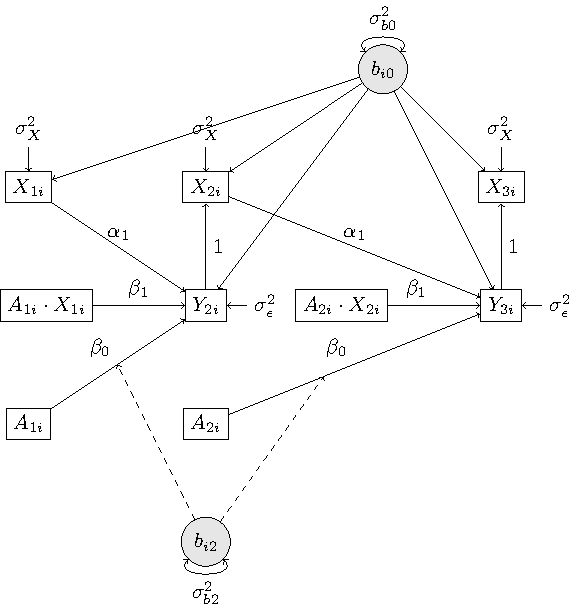
\includegraphics[width=1\textwidth,height=\textheight]{research-report_files/figure-pdf/fig-GMG_path-1.pdf}

}

\end{minipage}%
%
\begin{minipage}{0.50\linewidth}

\subcaption{\label{fig-GMA_path}GM A}

\centering{

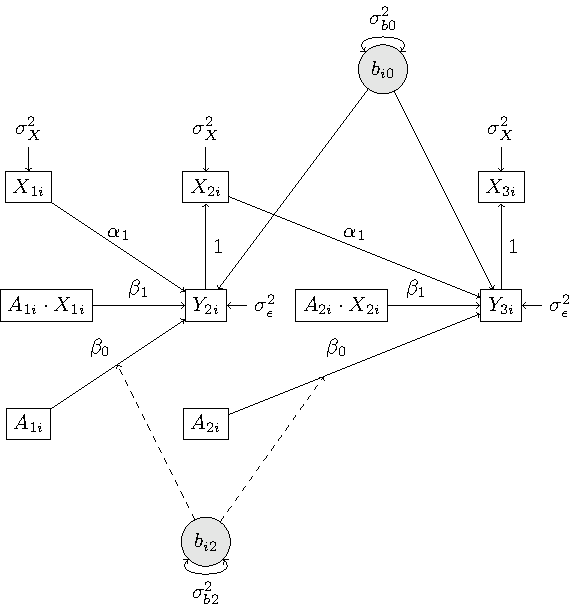
\includegraphics[width=1\textwidth,height=\textheight]{research-report_files/figure-pdf/fig-GMA_path-1.pdf}

}

\end{minipage}%
\newline
\begin{minipage}{0.50\linewidth}

\subcaption{\label{fig-GMB_path}GM B}

\centering{

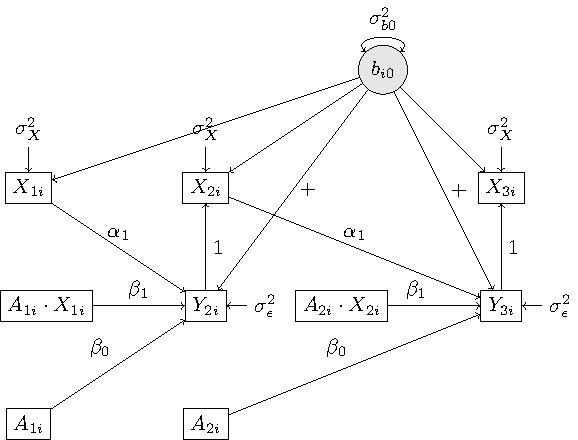
\includegraphics[width=1\textwidth,height=\textheight]{research-report_files/figure-pdf/fig-GMB_path-1.pdf}

}

\end{minipage}%
%
\begin{minipage}{0.50\linewidth}

\subcaption{\label{fig-GMC_path}GM C}

\centering{

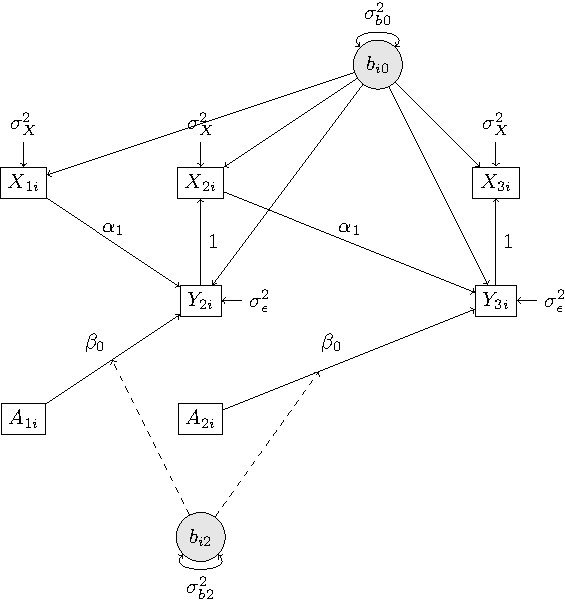
\includegraphics[width=1\textwidth,height=\textheight]{research-report_files/figure-pdf/fig-GMC_path-1.pdf}

}

\end{minipage}%
\newline
\begin{minipage}{0.50\linewidth}
\emph{Note.} Random effects are represented by grey circles, observed
variables by squares and relationships across variables by arrows, where
dashed lines are reserved for random slopes.\end{minipage}%

\end{figure}%

\subsection{Backdoor Criterion and
DAGs}\label{backdoor-criterion-and-dags}

According to the backdoor criterion (\citeproc{ref-pearl1988}{Pearl,
1988}, \citeproc{ref-pearl2009}{2009}), a requirement for causal
identification, causal effects can be identified by blocking non-causal
paths through conditioning on intermediate variables (e.g., controlling
or matching). If any non-causal paths cannot be blocked due to omitted
variables or measurement error, treatment and outcome remain linked via
backdoor paths, leading to biased estimates of the treatment effect
(\citeproc{ref-Kim2021a}{Kim \& Steiner, 2021}).

DAGs are a useful tool for representing causal relationships between
variables and to evaluate the assumptions needed for causal
identification (see \citeproc{ref-elwert2014}{Elwert \& Winship, 2014}
for a psychological example). We formulated the DAGs for the first three
observations of each generative model, where the random disturbance
\(b_{0i}\) was represented by the node U (e.g.,
\citeproc{ref-Kim2021a}{Kim \& Steiner, 2021}, see
Figure~\ref{fig-DAGs}).

When applying Pearl's backdoor criterion to the GMs, it may be observed
that there exists no backdoor path in the treatment effect
\(A_{it} \to Y_{it+1}\), as \(A_{it}\) does not have any parents. While
we need not control for covariate \(X_{it}\) to obtain an unbiased total
effect, doing so should not introduce bias. All things considered,
according to the backdoor criterion, controlling for the covariate
\(X_{it}\) should not result in biased estimates of the treatment effect
for any of the generative models.

\textbf{Note that these limitations of the DAG (not random effects or
interactions explicit) would have prevented us from evaluating the
conditional independence assumption.}

\begin{figure}[H]

\caption{\label{fig-DAGs}DAGs for Generative Models G, A, B and C (t =
1, 2, 3)}

\begin{minipage}{0.50\linewidth}

\subcaption{\label{fig-GMG_DAG}GM G, B, C}

\centering{

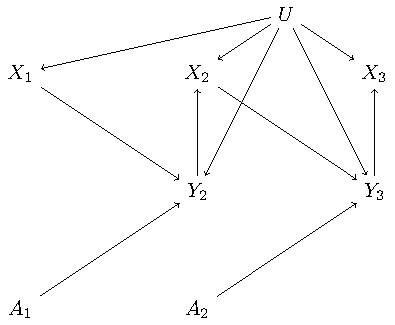
\includegraphics{research-report_files/figure-pdf/fig-GMG_DAG-1.pdf}

}

\end{minipage}%
%
\begin{minipage}{0.50\linewidth}

\subcaption{\label{fig-GMA_DAG}GM A}

\centering{

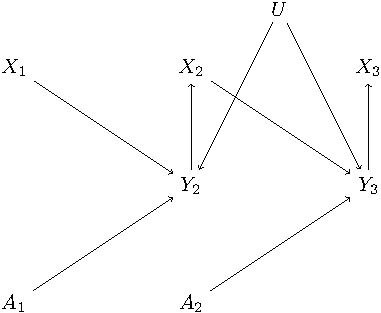
\includegraphics{research-report_files/figure-pdf/fig-GMA_DAG-1.pdf}

}

\end{minipage}%
\newline
\begin{minipage}{0.50\linewidth}
\emph{Note.} The red arrows show the biased backdoor path(s) in the
treatment efffect (before controlling for \(X_{it}\)).\end{minipage}%

\end{figure}%

\subsection{Simulation Study}\label{simulation-study}

Table~\ref{tbl-simulation-results} presents the simulation results for
each of the generative and analytical models. The estimates for the
analytical MLM may be interpreted in terms of bias, where given the
value of the treatment effect \(\beta_0 = 1\), absolute bias of .05
would imply \(5\%\) relative bias. Here we find the greatest absolute
bias of \(.02-.06\) for GM3, \(\leq .015\) for GM1/2, \(\leq .010\) for
GM3B and , \(\leq .005\) for GM3A. While the bias found for the original
GMs 1, 2 and 3 was slightly larger here compared to Qian et al.
(\citeproc{ref-qian2020}{2020}), the overall pattern remained the same.
To conclude, once we remove either the dependency of the random
intercept with the covariate (GM1), the random slope \(b_{i2}\) (GM3A)
or the interaction \(\beta_1\) (GM3B) from GM3, the bias dissapears or
becomes very small. The bias in GM3 decreases as the number of
timepoints \(T\) increases from 10 to 30. Note that the MLM model
fitting success rates are particularly poor for GM2, where in the worst
case, only 87 of the 1000 models were fitted.

\begin{table}

\caption{\label{tbl-simulation-results}Treatment effect bias for
Generative Models G, A, B and C over 1000 replications}

\centering{

\begin{tabu} to \linewidth {>{\raggedright\arraybackslash}p{5em}>{\raggedleft}X>{\raggedleft}X>{\raggedleft}X>{\raggedleft}X>{\raggedleft}X}
\toprule
\multicolumn{3}{c}{ } & \multicolumn{2}{c}{$\beta_0$} & \multicolumn{1}{c}{ } \\
\cmidrule(l{3pt}r{3pt}){4-5}
GM & T & N & Bias & SD & SR\\
\midrule
 &  & 30 & -0.052 & 0.245 & 0.999\\
\cmidrule{3-6}
 &  & 100 & -0.064 & 0.134 & 1.000\\
\cmidrule{3-6}
 & \multirow{-3}{*}{\raggedleft\arraybackslash 10} & 200 & -0.051 & 0.096 & 1.000\\
\cmidrule{2-6}
 &  & 30 & -0.024 & 0.206 & 0.997\\
\cmidrule{3-6}
 &  & 100 & -0.030 & 0.108 & 0.996\\
\cmidrule{3-6}
\multirow{-6}{5em}[0.5\dimexpr\aboverulesep+\belowrulesep+\cmidrulewidth]{\raggedright\arraybackslash G} & \multirow{-3}{*}{\raggedleft\arraybackslash 30} & 200 & -0.023 & 0.080 & 0.997\\
\cmidrule{1-6}
 &  & 30 & 0.000 & 0.238 & 0.998\\
\cmidrule{3-6}
 &  & 100 & -0.012 & 0.129 & 1.000\\
\cmidrule{3-6}
 & \multirow{-3}{*}{\raggedleft\arraybackslash 10} & 200 & 0.003 & 0.093 & 0.999\\
\cmidrule{2-6}
 &  & 30 & -0.001 & 0.203 & 0.998\\
\cmidrule{3-6}
 &  & 100 & -0.007 & 0.107 & 0.996\\
\cmidrule{3-6}
\multirow{-6}{5em}[0.5\dimexpr\aboverulesep+\belowrulesep+\cmidrulewidth]{\raggedright\arraybackslash A} & \multirow{-3}{*}{\raggedleft\arraybackslash 30} & 200 & 0.001 & 0.079 & 0.996\\
\cmidrule{1-6}
 &  & 30 & 0.000 & 0.126 & 1.000\\
\cmidrule{3-6}
 &  & 100 & 0.004 & 0.073 & 1.000\\
\cmidrule{3-6}
 & \multirow{-3}{*}{\raggedleft\arraybackslash 10} & 200 & 0.002 & 0.048 & 1.000\\
\cmidrule{2-6}
 &  & 30 & -0.001 & 0.071 & 1.000\\
\cmidrule{3-6}
 &  & 100 & 0.000 & 0.040 & 1.000\\
\cmidrule{3-6}
\multirow{-6}{5em}[0.5\dimexpr\aboverulesep+\belowrulesep+\cmidrulewidth]{\raggedright\arraybackslash B} & \multirow{-3}{*}{\raggedleft\arraybackslash 30} & 200 & 0.000 & 0.028 & 1.000\\
\cmidrule{1-6}
 &  & 30 & 0.001 & 0.217 & 0.999\\
\cmidrule{3-6}
 &  & 100 & -0.008 & 0.121 & 1.000\\
\cmidrule{3-6}
 & \multirow{-3}{*}{\raggedleft\arraybackslash 10} & 200 & 0.005 & 0.087 & 1.000\\
\cmidrule{2-6}
 &  & 30 & 0.000 & 0.193 & 1.000\\
\cmidrule{3-6}
 &  & 100 & -0.008 & 0.103 & 0.997\\
\cmidrule{3-6}
\multirow{-6}{5em}[0.5\dimexpr\aboverulesep+\belowrulesep+\cmidrulewidth]{\raggedright\arraybackslash C} & \multirow{-3}{*}{\raggedleft\arraybackslash 30} & 200 & 0.001 & 0.075 & 0.999\\
\bottomrule
\end{tabu}

\emph{Note.} GM: generative model. T: number of timepoints. N: sample
size. SD: standard deviation of estimates across replications. SR: model
fitting success rate. Bias: \(\hat{\beta}_{0,MLM} - \beta_{0,MLM}\).

}

\end{table}%

\begin{figure}[H]

\caption{\label{fig-simulation-results}Estimation bias for the fixed
treatment effect \(\beta_0\) of each generative model for different
combinations of sample size N and number of timepoints T over 1000
simulation replications}

\begin{minipage}{0.50\linewidth}

\subcaption{\label{fig-simulation-results-1}T=10, N=30}

\centering{

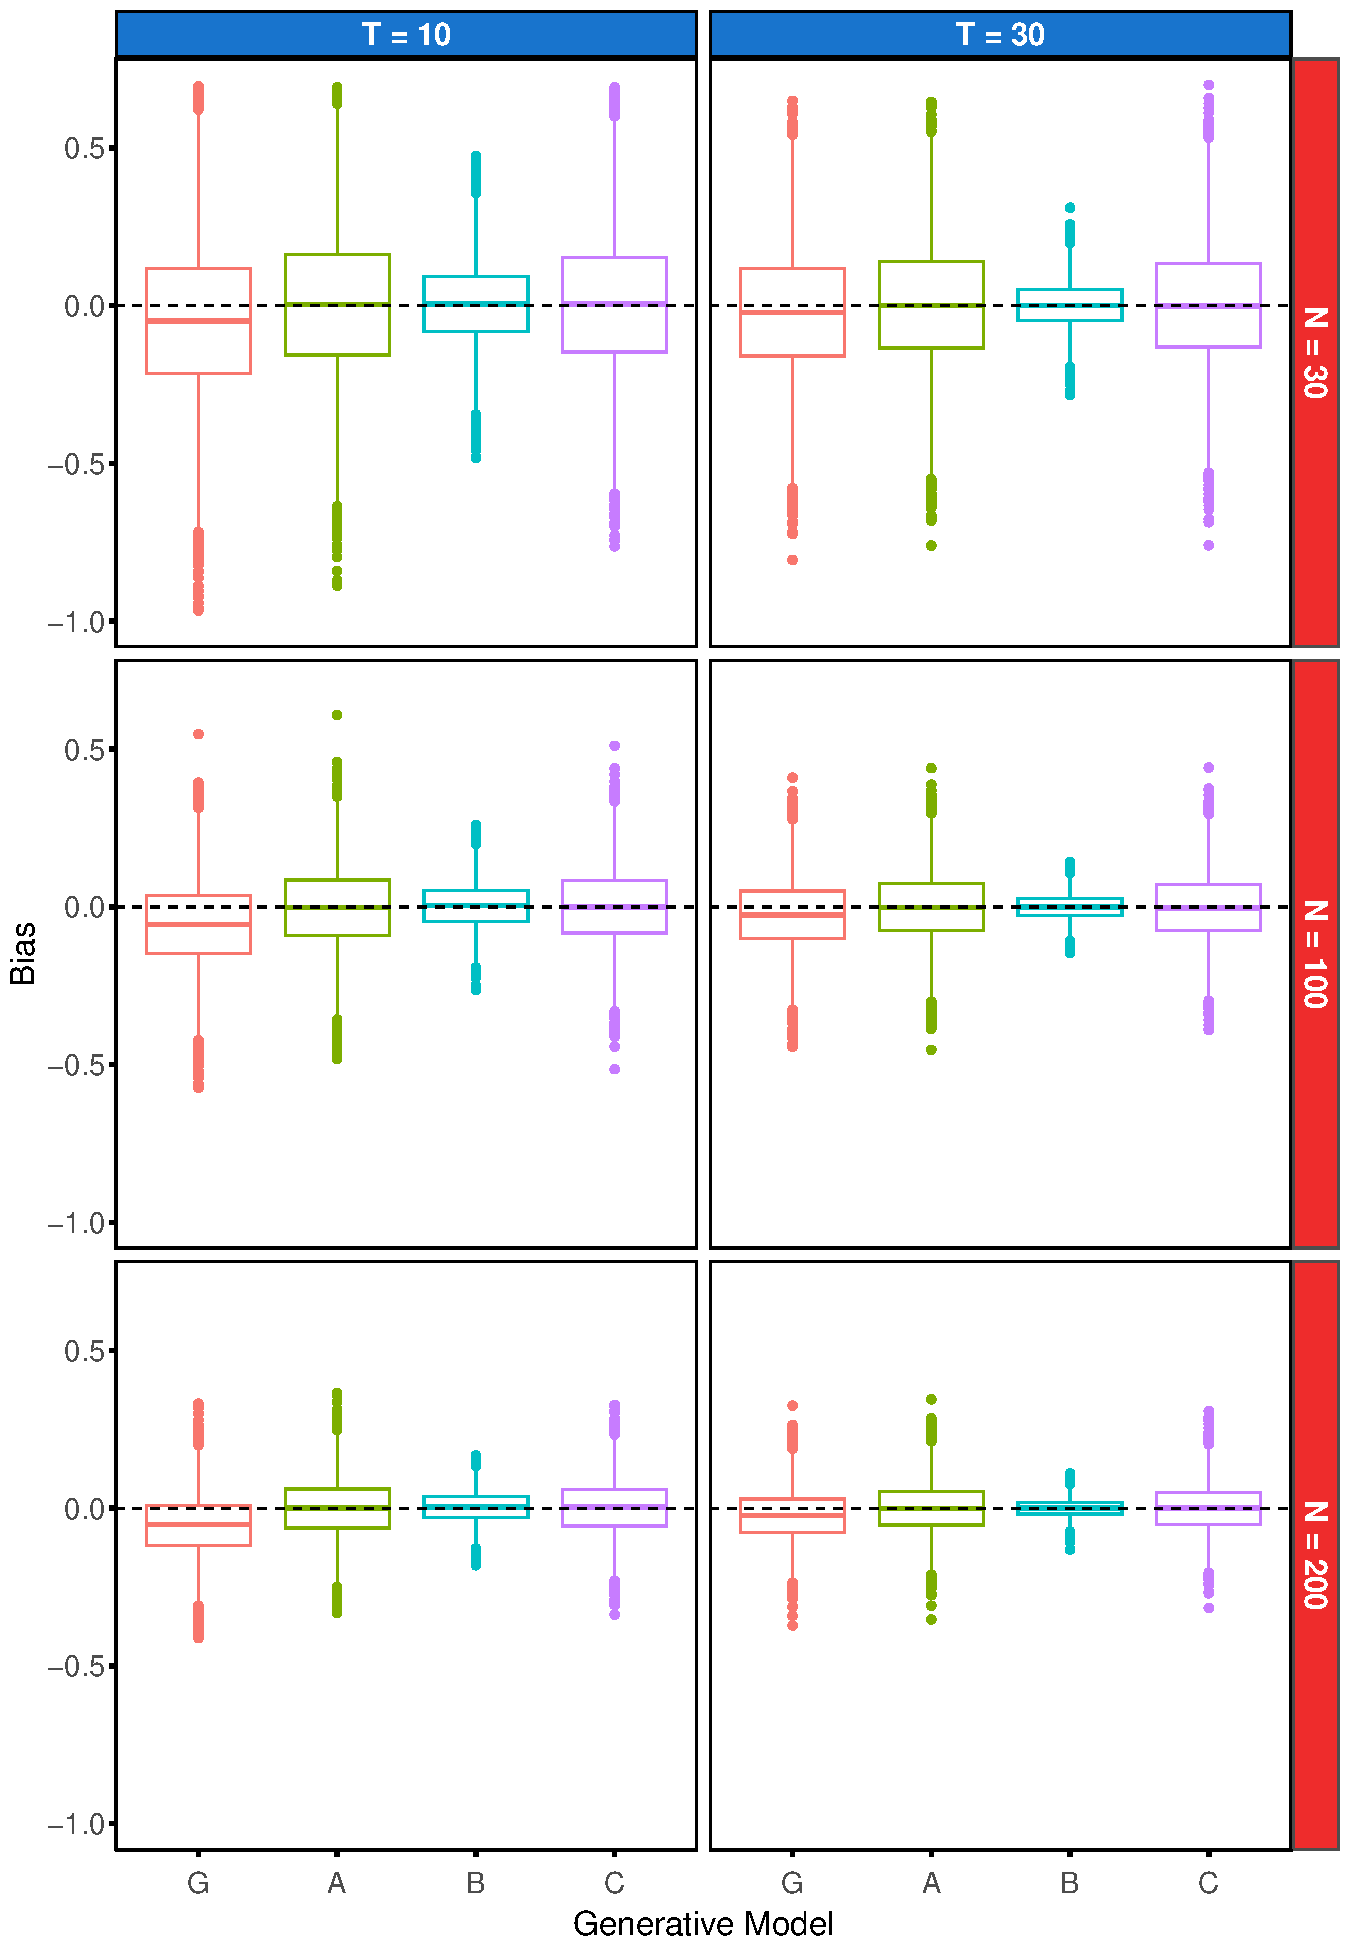
\includegraphics{research-report_files/figure-pdf/fig-simulation-results-1.pdf}

}

\end{minipage}%
%
\begin{minipage}{0.50\linewidth}

\subcaption{\label{fig-simulation-results-2}T=10, N=100}

\centering{

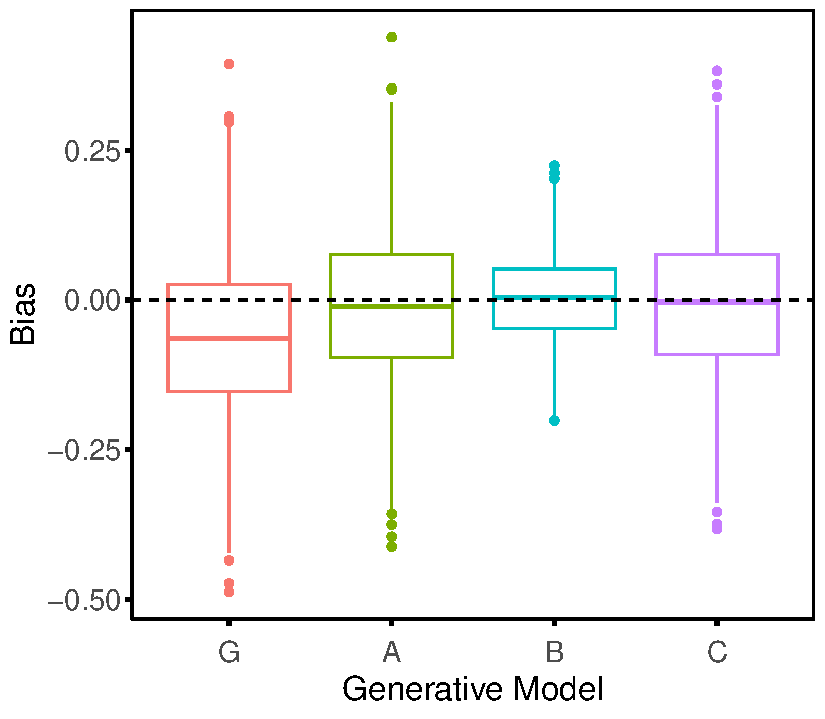
\includegraphics{research-report_files/figure-pdf/fig-simulation-results-2.pdf}

}

\end{minipage}%
\newline
\begin{minipage}{0.50\linewidth}

\subcaption{\label{fig-simulation-results-3}T=10, N=200}

\centering{

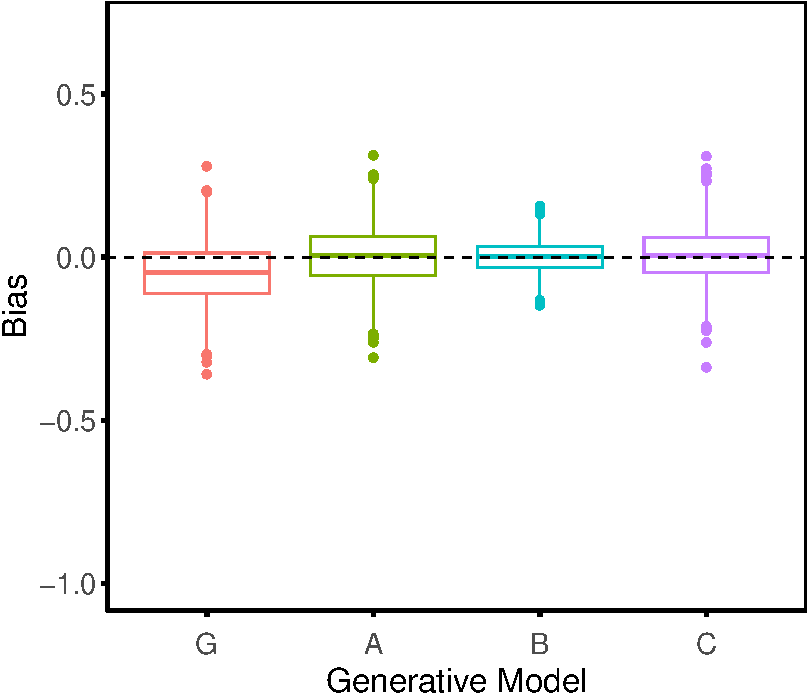
\includegraphics{research-report_files/figure-pdf/fig-simulation-results-3.pdf}

}

\end{minipage}%
%
\begin{minipage}{0.50\linewidth}

\subcaption{\label{fig-simulation-results-4}T=30, N=30}

\centering{

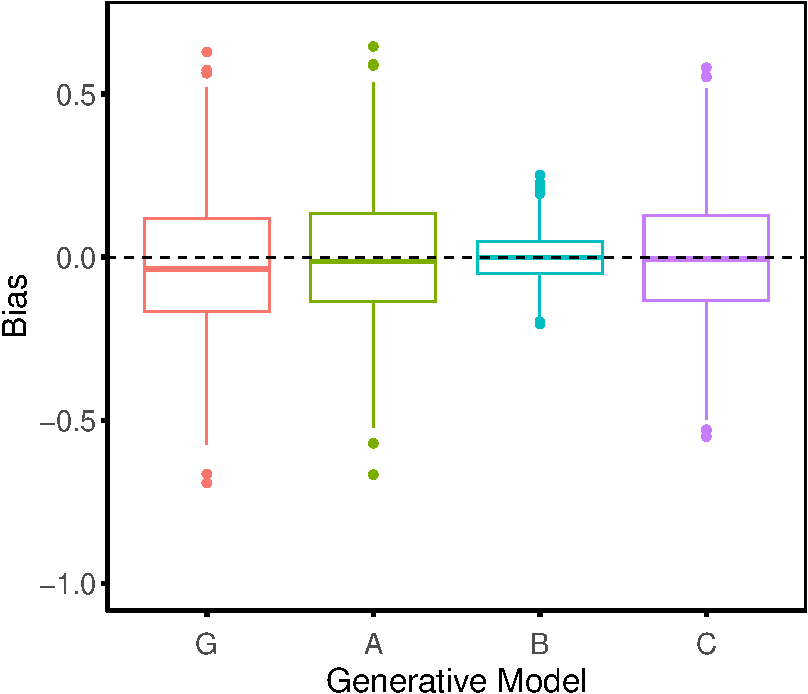
\includegraphics{research-report_files/figure-pdf/fig-simulation-results-4.pdf}

}

\end{minipage}%
\newline
\begin{minipage}{0.50\linewidth}

\subcaption{\label{fig-simulation-results-5}T=30, N=100}

\centering{

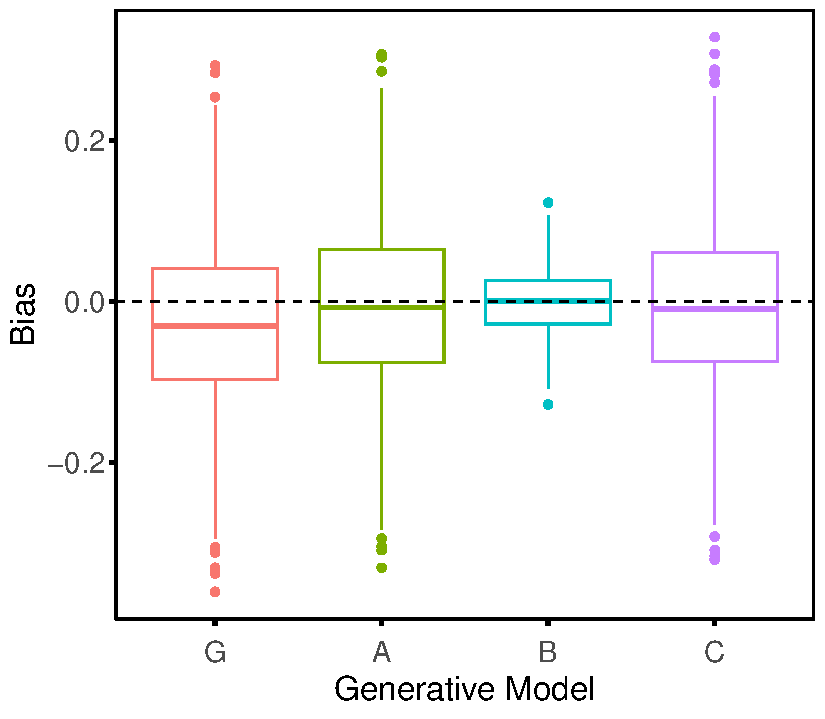
\includegraphics{research-report_files/figure-pdf/fig-simulation-results-5.pdf}

}

\end{minipage}%
%
\begin{minipage}{0.50\linewidth}

\subcaption{\label{fig-simulation-results-6}T=30, N=200}

\centering{

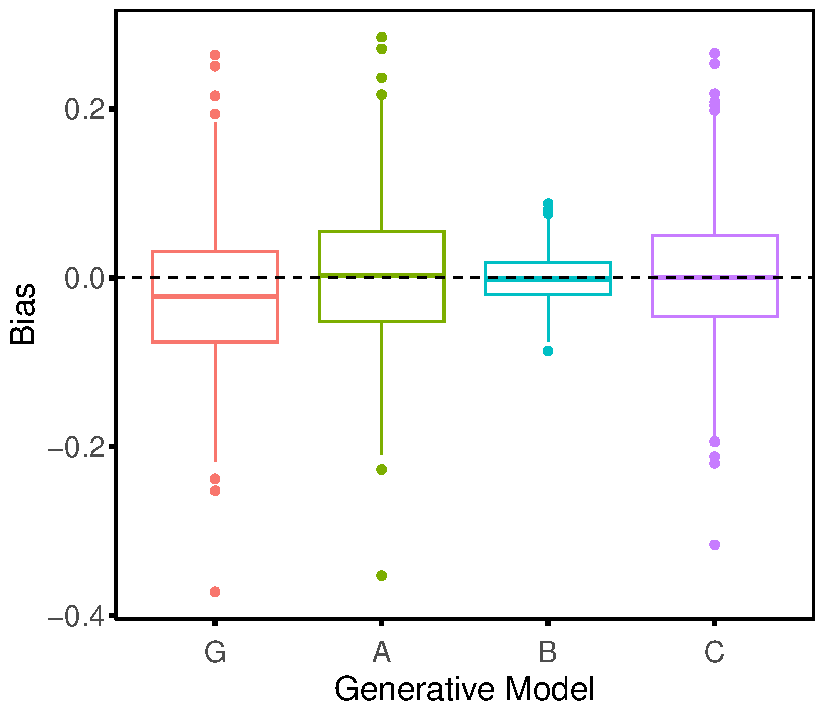
\includegraphics{research-report_files/figure-pdf/fig-simulation-results-6.pdf}

}

\end{minipage}%

\end{figure}%

\section{Discussion}\label{discussion}

This report employed both graphical methods and data simulations to
understand and explain the issue of endogenous covariates. Now we first
discuss the expected results based on the backdoor criterion Pearl
(\citeproc{ref-pearl2009}{2009}) and the conditional independence
assumption (\citeproc{ref-qian2020}{Qian et al., 2020}), whereafter we
discuss the findings relating to the two research questions.

Using the conditional independence assumption of Qian et al.
(\citeproc{ref-qian2020}{2020}), we would expect, based on the path
diagrams, that the treatment effect would be biased for GM3, 3A and 3B.
On the other hand, the backdoor criterion suggested the absence of bias
for all generative models. While Qian et al.
(\citeproc{ref-qian2020}{2020}) show that GM3 is the only model with
bias in the treatment effect, the backdoor criterion failed to identify
this bias, as there is no backdoor path in the treatment effect. This
may be explained by the fact that the classic DAG does not impose
restrictions based on (a) the random slopes and (b) interaction effects.

The first research question---pertaining to the extent of treatment
effect bias in MLM estimates of generative model that were nested in
GM3---was investigated using the analytical multilevel model. First, we
reproduced the findings by Qian et al. (\citeproc{ref-qian2020}{2020})
who found consistent estimators for GM1 and and inconsistent ones for
GM3. Using additional generative models, we found that bias became
indiscernable when removing from GM3 either the dependency between the
random intercept and covariate (GM1), the random slope for treatment
(GM3A) or the interaction effect (GM3B). This finding is in sharp
contrast to the suggestion of the conditional independence assumption
that the treatment effect would be biased for GM3, 3A and 3B.

The current research report leaves several avenues unexplored. First, it
is unclear whether the simulation findings pertaining the generative
models in Qian et al. (\citeproc{ref-qian2020}{2020}) and here
generalize to other generative models. For instance, we found here that
removal of a random slope or interaction from GM3 got rid of most if not
all of the treatment effect bias. Thus, it is important to establish how
this generalizes, so that practical recommendations can be formulated.
This is particularly important, since while violations of model
assumptions are never desired, the robustness against and the practical
implications of a violation is what matters. Second, it is unclear how
exactly the divide between the literatures pertaining to the focus of
the MLM on different centering methods and within- and between-person
interpretations and the focus of the GEE on marginal and conditional
interpretations may be bridged. Consequently, future research could
assess the implications of centering methods in MLMs on the extent to
which the marginal interpretation of MLM breaks down. Third, we found
that the classical DAG may not be sufficient to identify bias in the
treatment effect for GM3, especially due to its lack of specification of
interaction effects. Concerns regarding the use of Pearl's backdoor
criterion in situations with interaction effects have been voiced by
several people (see Weinberg (\citeproc{ref-weinberg2007}{2007}); Attia
et al. (\citeproc{ref-attia2022}{2022})). Future research could explore
to what extent proposed extensions of the DAG may be useful in
identifying bias in the treatment effect for GM3. Finally, it may be
interesting to investigate the implications of endogenous covariates in
MLMs for other types of longitudinal data analysis methods, such as
dynamic structural equation modelling (DSEM; a widely used framework in
the social sciences based on MLM).

Third, since the issue extends to all longitudinal data analysis methods
according to Diggle (\citeproc{ref-diggle2002}{2002}), in future
research it may be interesting to investigate the implications of
endogenous covariates in MLMs for other types of longitudinal data
analysis methods, such as dynamic structural equation modelling (DSEM; a
widely used framework in the social sciences based on MLM).

\newpage

\section{References}\label{references}

\phantomsection\label{refs}
\begin{CSLReferences}{1}{0}
\bibitem[\citeproctext]{ref-attia2022}
Attia, J., Holliday, E., \& Oldmeadow, C. (2022). A proposal for
capturing interaction and effect modification using DAGs.
\emph{International Journal of Epidemiology}, \emph{51}(4), 1047--1053.
\url{https://doi.org/10.1093/ije/dyac126}

\bibitem[\citeproctext]{ref-bates2015}
Bates, D., Mächler, M., Bolker, B., \& Walker, S. (2015). Fitting linear
mixed-effects models using {lme4}. \emph{Journal of Statistical
Software}, \emph{67}(1), 148.
\url{https://doi.org/10.18637/jss.v067.i01}

\bibitem[\citeproctext]{ref-bauer2011}
Bauer, D. J., \& Sterba, S. K. (2011). Fitting multilevel models with
ordinal outcomes: Performance of alternative specifications and methods
of estimation. \emph{Psychological Methods}, \emph{16}(4), 373--390.
\url{https://doi.org/10.1037/a0025813}

\bibitem[\citeproctext]{ref-daniel2013}
Daniel, R. m., Cousens, S. n., De Stavola, B. l., Kenward, M. G., \&
Sterne, J. a. C. (2013). Methods for dealing with time-dependent
confounding. \emph{Statistics in Medicine}, \emph{32}(9), 1584--1618.
\url{https://doi.org/10.1002/sim.5686}

\bibitem[\citeproctext]{ref-diggle2002}
Diggle, P. (2002). \emph{Analysis of Longitudinal Data}. OUP Oxford.

\bibitem[\citeproctext]{ref-elwert2014}
Elwert, F., \& Winship, C. (2014). Endogenous selection bias: The
problem of conditioning on a collider variable. \emph{Annual Review of
Sociology}, \emph{40}, 31--53.
\url{https://doi.org/10.1146/annurev-soc-071913-043455}

\bibitem[\citeproctext]{ref-hamaker2020}
Hamaker, E. L., \& Muthén, B. (2020). The fixed versus random effects
debate and how it relates to centering in multilevel modeling.
\emph{Psychological Methods}, \emph{25}(3), 365--379.
\url{https://doi.org/10.1037/met0000239}

\bibitem[\citeproctext]{ref-Kim2021a}
Kim, Y., \& Steiner, P. M. (2021). Causal graphical views of fixed
effects and random effects models. \emph{British Journal of Mathematical
and Statistical Psychology}, \emph{74}(2), 165--183.
\url{https://doi.org/10.1111/bmsp.12217}

\bibitem[\citeproctext]{ref-pearl1988}
Pearl, J. (1988). \emph{Probabilistic Reasoning in Intelligent Systems:
Networks of Plausible Inference}. Morgan Kaufmann.

\bibitem[\citeproctext]{ref-pearl2009}
Pearl, J. (2009). \emph{Causality: Models, reasoning, and inference}
(2nd ed.). Cambridge University Press.

\bibitem[\citeproctext]{ref-qian2020}
Qian, T., Klasnja, P., \& Murphy, S. A. (2020). Linear mixed models with
endogenous covariates: Modeling sequential treatment effects with
application to a mobile health study. \emph{Statistical Science : A
Review Journal of the Institute of Mathematical Statistics},
\emph{35}(3), 375--390. \url{https://doi.org/10.1214/19-sts720}

\bibitem[\citeproctext]{ref-raudenbush2002}
Raudenbush, S. W., \& Bryk, A. S. (2002). \emph{Hierarchical Linear
Models: Applications and Data Analysis Methods} (2nd ed.). SAGE.

\bibitem[\citeproctext]{ref-Schoot2017}
Schoot, J. H. M. M. R. van de. (2017). \emph{Multilevel analysis:
Techniques and applications, third edition} (3rd ed.). Routledge.
\url{https://doi.org/10.4324/9781315650982}

\bibitem[\citeproctext]{ref-rcoreteam2024}
Team, R. C. (2024). \emph{R: A language and environment for statistical
computing}. R Foundation for Statistical Computing.
\url{https://www.R-project.org/}

\bibitem[\citeproctext]{ref-weinberg2007}
Weinberg, C. R. (2007). Commentary: Can DAGs clarify effect
modification? \emph{Epidemiology}, \emph{18}(5), 569--572.
\url{https://www.jstor.org/stable/20486428}

\end{CSLReferences}




\end{document}
